% !TEX root = ../DML_report.tex
\section{Ход работы}

По итогам предыдущей работы была разработана модифицированная SQL-схема БД для музыкальной библиотеки (\vref{pic:scheme}).

\begin{figure}[ht]
	\centering
	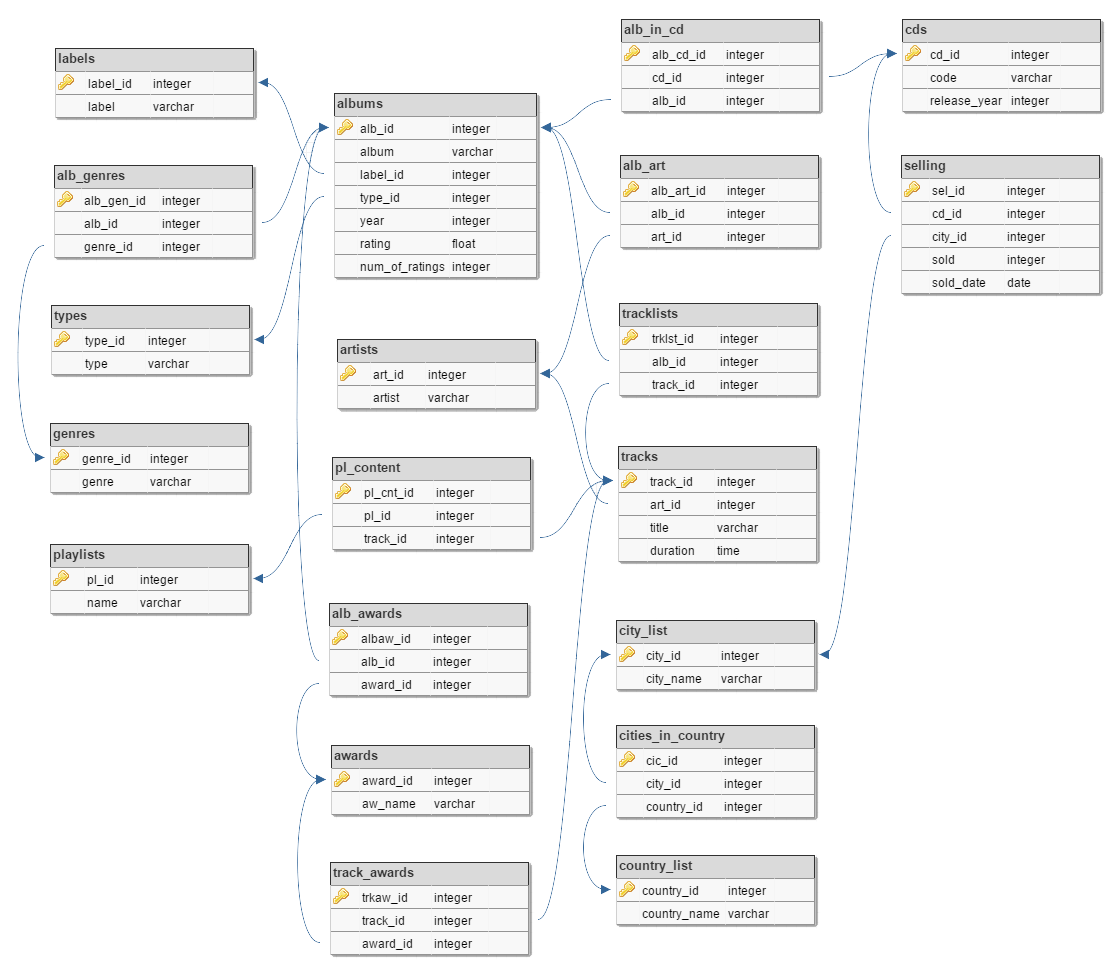
\includegraphics[width=\textwidth]{scheme_m}
	\caption{SQL-схема БД}
	\label{pic:scheme}
\end{figure}

Будем использовать данную БД для выполнения работы. В процессе будем создавать представления и ХП в соответствии с заданием, за исключением тех случаев, где в этом нет необходимости.

\subsection{Стандартные запросы}

\subsubsection{Сделать выборку всех данных из каждой таблицы}

\lstinputlisting[language=SQL, morekeywords={REFERENCES}]{code/1.sql}

\subsubsection{Сделать выборку данных из одной таблицы при нескольких условиях, с использованием логических операций LIKE, BETWEEN, IN (не менее 3-х разных примеров)}

\lstinputlisting[language=SQL, morekeywords={REFERENCES}]{code/2.sql}

\subsubsection{Создать в запросе вычисляемое поле}

\lstinputlisting[language=SQL, morekeywords={REFERENCES, to, DATEDIFF}]{code/3.sql}

\subsubsection{Сделать выборку всех данных с сортировкой по нескольким полям}

\lstinputlisting[language=SQL, morekeywords={REFERENCES, to}]{code/4.sql}

\subsubsection{Создать запрос, вычисляющий несколько совокупных характеристик таблиц}

\lstinputlisting[language=SQL, morekeywords={REFERENCES, to, DATEDIFF}]{code/5.sql}

\subsubsection{Сделать выборку данных из связанных таблиц (не менее двух примеров)}

\lstinputlisting[language=SQL, morekeywords={REFERENCES, to}]{code/6.sql}

\subsubsection{Создать запрос, рассчитывающий совокупную характеристику с использованием группировки, наложите ограничение на результат группировки}

\lstinputlisting[language=SQL, morekeywords={REFERENCES, to}]{code/7.sql}

\subsubsection{Придумать и реализовать пример использования вложенного запроса}

\lstinputlisting[language=SQL, morekeywords={REFERENCES, to}]{code/8.sql}

\subsubsection{С помощью оператора INSERT добавить в каждую таблицу по одной записи}

\lstinputlisting[language=SQL, morekeywords={REFERENCES, to, PROCEDURE, BEGIN}]{code/9.sql}

\subsubsection{С помощью оператора UPDATE изменить значения нескольких полей у всех записей, отвечающих заданному условию}

\lstinputlisting[language=SQL, morekeywords={REFERENCES, to, PROCEDURE, BEGIN}]{code/10.sql}

\subsubsection{С помощью оператора DELETE удалить запись, имеющую максимальное (минимальное) значение некоторой совокупной характеристики}

\lstinputlisting[language=SQL, morekeywords={REFERENCES, to, PROCEDURE, BEGIN}]{code/11.sql}

\subsubsection{С помощью оператора DELETE удалить записи в главной таблице, на которые не ссылается подчиненная таблица (используя вложенный запрос)}

\lstinputlisting[language=SQL, morekeywords={REFERENCES, to, PROCEDURE, BEGIN}]{code/12.sql}

\subsection{Индивидуальное задание}

\subsubsection{Вывести 5 лейблов, треки, с альбомов которых, наиболее часто встречаются в плейлистах}

\lstinputlisting[language=SQL, morekeywords={REFERENCES, to, PROCEDURE}]{code/ind1.sql}

\subsubsection{Вывести треки, которые содержатся в альбомах, записанных на заданных лейблах или относящихся к заданным жанрам}

\lstinputlisting[language=SQL, morekeywords={REFERENCES, to, PROCEDURE, BEGIN}]{code/ind2.sql}

\subsubsection{Для каждого жанра вывести отношение количества появления треков в плейлистах к количеству альбомов, на которых содержатся треки данного жанра}

\lstinputlisting[language=SQL, morekeywords={REFERENCES, to, PROCEDURE, BEGIN}]{code/ind3.sql}